% 1959 — A3 poster for LPM 2026 Rome (AV Installation, program #1959)
% Build: make            (xelatex, twice for the footer/last-page refs)
%
% The installation text is the accepted LPM program description,
% lightly copy-edited. The chip photograph is the annotated die
% micrograph used in the papers (fig/die.jpg, copied from
% paper/RISCV_NeuronArray_2026/figures/).

\documentclass[11pt]{article}

\usepackage[paperwidth=297mm,paperheight=420mm,
            left=22mm,right=22mm,top=20mm,bottom=20mm]{geometry}
\usepackage{fontspec}
\usepackage{graphicx}
\usepackage{xcolor}
\usepackage{paracol}
\usepackage{lettrine}

% Work Sans: the typeface of the LPM 2026 Rome site. TTF files are kept
% next to this source so the build does not depend on system fontconfig.
\setmainfont{WorkSans}[
  Path           = fonts/,
  Extension      = .ttf,
  UprightFont    = WorkSans-Regular,
  ItalicFont     = WorkSans-Italic,
  BoldFont       = WorkSans-Bold,
  BoldItalicFont = WorkSans-BoldItalic,
]

% ---------- palette: LPM 2026 Rome brand ----------
% red #9a1915 and black #000 taken from the LPM site stylesheet
% (combo.lpm.2026-rome.min.css); paper is white.
\definecolor{ink}{HTML}{000000}      % black
\definecolor{spike}{HTML}{9A1915}    % LPM red
\definecolor{faint}{HTML}{9A1915}    % LPM red, for kicker & captions

\color{ink}
\pagestyle{empty}
\setlength{\parindent}{0pt}
\setlength{\parskip}{0.8em}
\setlength{\columnsep}{9mm}
\columnratio{0.58}
\hyphenpenalty=10000
\exhyphenpenalty=10000
\setlength{\emergencystretch}{3em}

% ---------- helpers ----------
\newcommand{\kicker}[1]{{\fontsize{10.5}{14}\selectfont\color{faint}%
  \addfontfeature{LetterSpace=12.0}\MakeUppercase{#1}}}
\newcommand{\captionfont}{\fontsize{10.5}{13.0}\selectfont\color{faint}}
\newcommand{\hruleink}{\par\vspace{1.5em}{\color{spike}\rule{\linewidth}{0.55pt}}\par\vspace{1.5em}}

\begin{document}

% ================= header =================
\begin{center}
  {\kicker{LPM 2026 Rome — Live Performers Meeting}}\\[0.5em]
  {\kicker{MAM — Media Art Museum \,\textbar\, 22--25 October 2026}}\\[2.2em]
  {\fontsize{142}{126}\selectfont\bfseries\color{spike}1959}\\[1.7em]
  {\fontsize{21}{26}\selectfont An audio-visual installation\ \ \textperiodcentered\ \ \ Federico Corradi}
\end{center}
\vspace{0.5em}
\hruleink

% ================= body =================
\begin{paracol}{2}

% -------- left column: the piece --------
\fontsize{14.2}{18.8}\selectfont

\lettrine[lines=2,findent=2pt,nindent=0pt]{I}{n} 1959, David Hubel and Torsten
Wiesel lowered an electrode into the visual cortex of a cat and moved a bar of
light across its field of view. A single neuron answered, and its spikes were
audible as clicks on tape. They received the 1981 Nobel Prize for what those
clicks meant: that seeing is built, cell by cell, from single features of the
world.

This installation plays that recording into a mixed-signal chip I designed and
fabricated, containing sixteen analog spiking neurons. Each neuron has a
membrane, a leak and a threshold. It has no clock and computes no numbers: it
answers in continuous time, in physics. It does not answer identically. No two
neurons, born or made, ever do.

The visitor hears both: a cat's cortex from 1959 and a silicon analog neuron
from 2026, made with state-of-the-art microelectronics, in the same room,
sixty-seven years apart, almost in unison. The chip is exposed on a plinth
beside a print of the neuron and synapse layout.

Those same clicks are where machine vision began. Today's neural networks are
a diagram of this cat. What they copied was the wiring. What they left behind
was the body.

Sixteen neurons is not a brain. It is the start of a different bet: that
machines which have to perceive, in real time, in the world, on the power the
world can spare, should be made of physics rather than numbers. How far that
goes, nobody knows yet. In 1959, nobody knew either.

\vspace{1.6em}
{\color{spike}\rule{\linewidth}{0.55pt}}
\vspace{1.6em}

{\fontsize{21}{26}\selectfont\itshape
What they copied was the wiring. \textcolor{spike}{What they left behind was
the body.}}

\switchcolumn

% -------- right column: the cat, then the chip --------
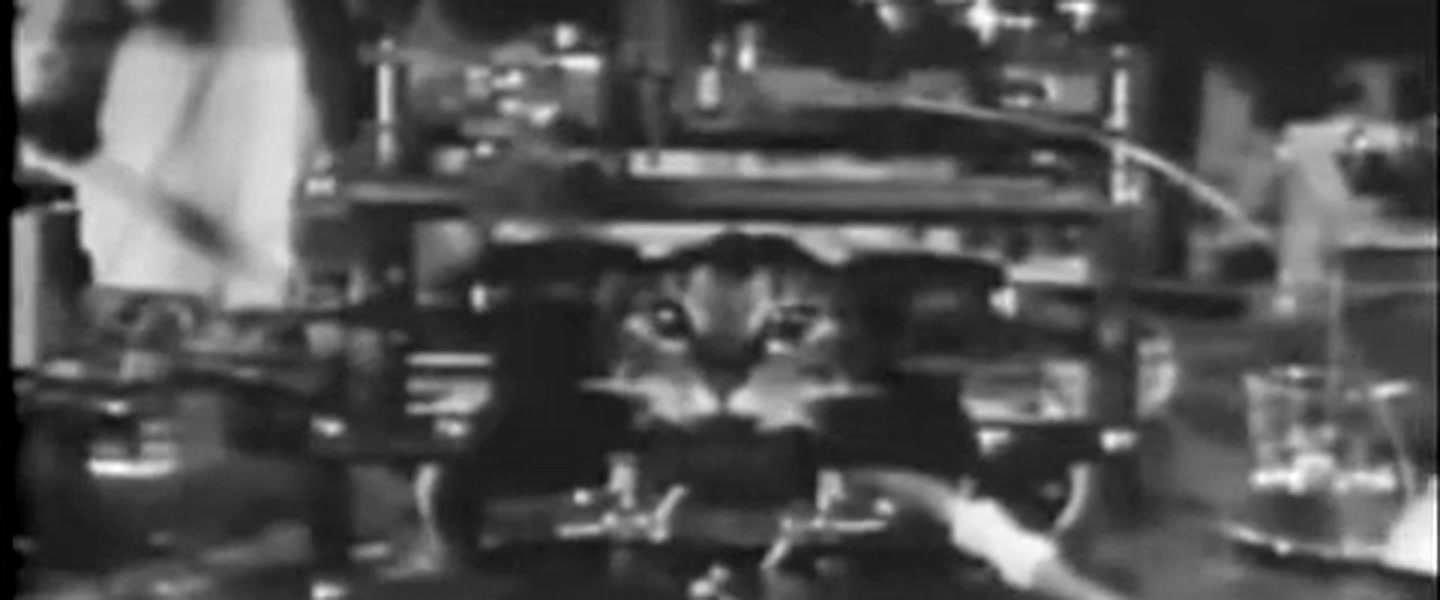
\includegraphics[width=0.94\linewidth]{fig/cat_1959.jpg}

\vspace{0.8em}
{\captionfont
\textbf{The cat, 1959.} Electrode in the visual cortex, spikes on a
loudspeaker. \textit{Still: ``Hubel \& Wiesel 2: Cat Experiment''.}}

\vspace{0.8em}
\centerline{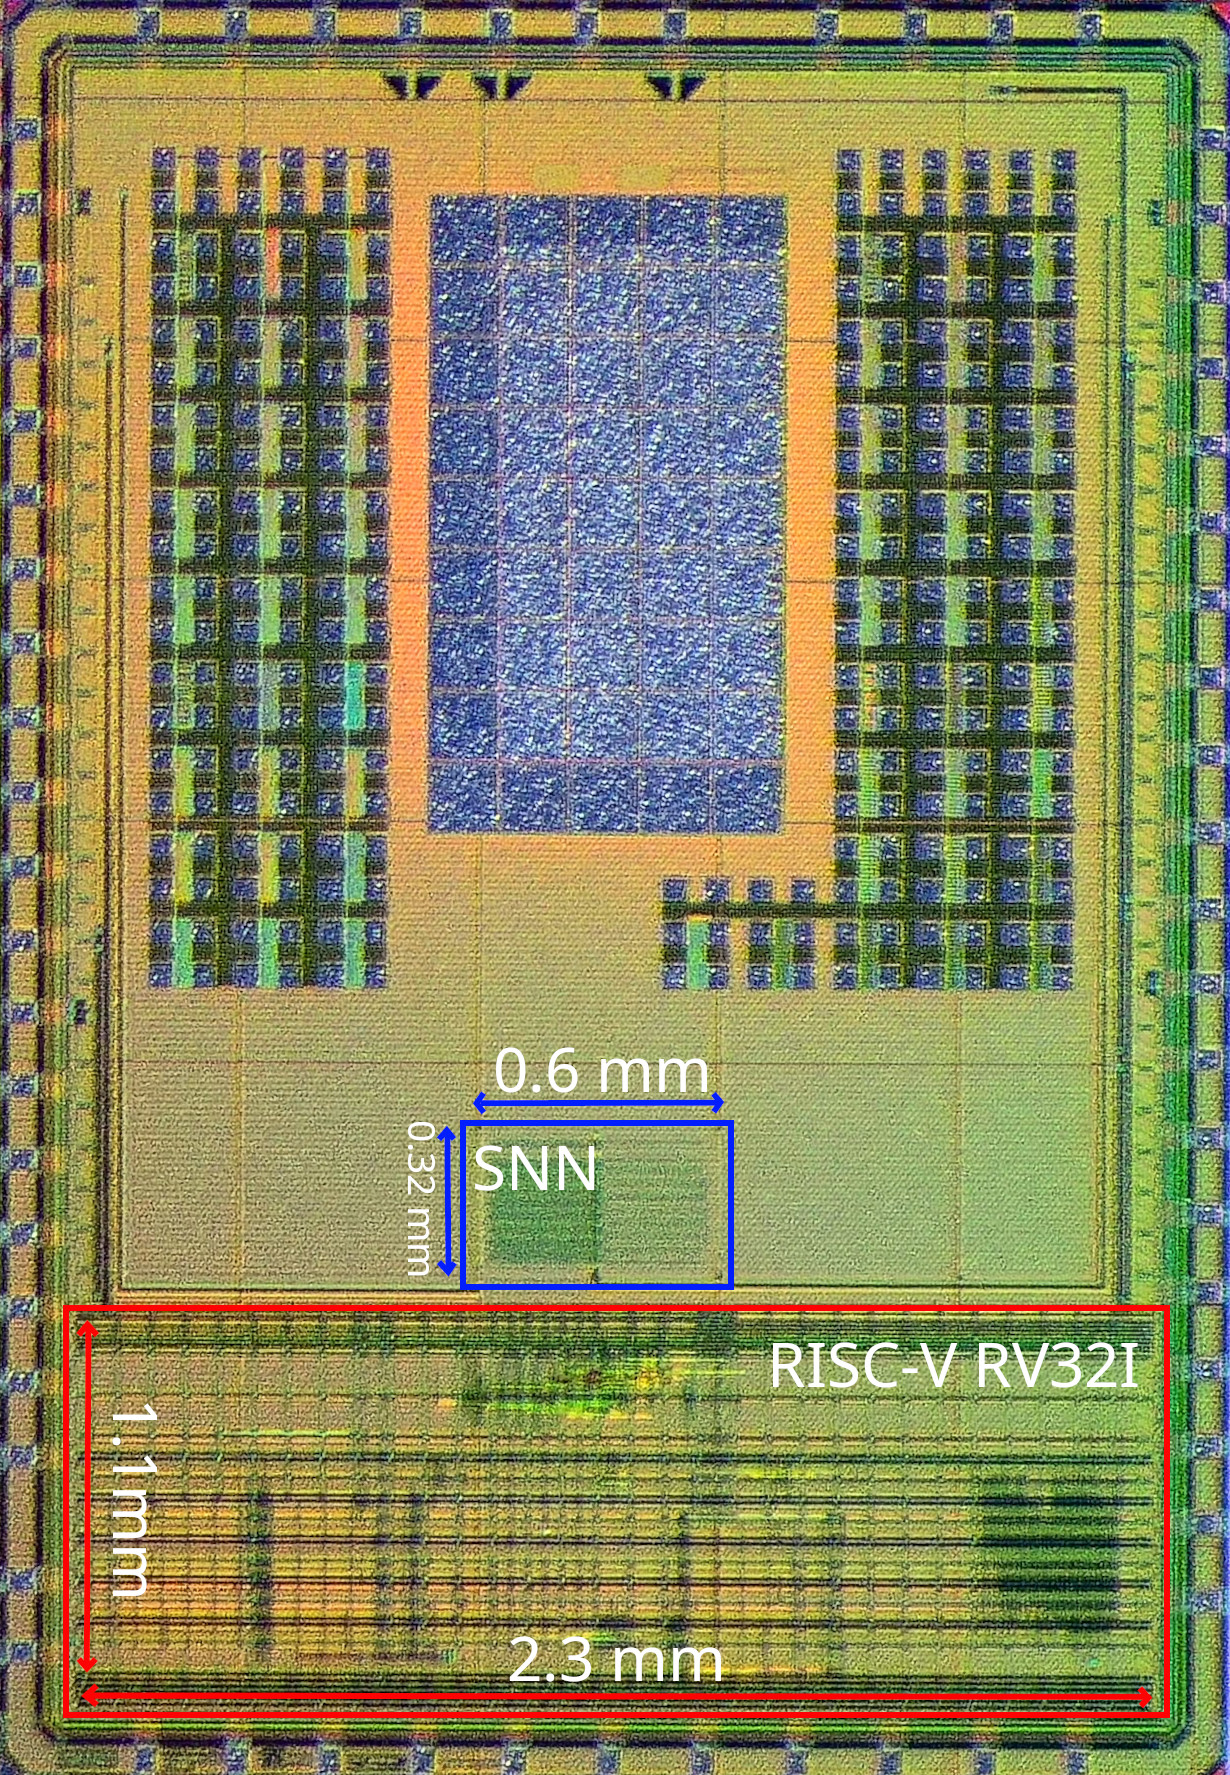
\includegraphics[width=0.60\linewidth]{fig/die.jpg}}

\vspace{0.9em}
{\captionfont
\textbf{The chip under a microscope.} A small computer and sixteen artificial
neurons on one piece of silicon just \textbf{3.6 × 5.2 mm}. Like the
cat's, these neurons run on current, not numbers. What you hear is one neuron's
voltage, amplified straight from the chip --- no computer in between.}

\vspace{0.6em}
{\color{spike}\rule{\linewidth}{0.55pt}}
\vspace{0.7em}

\kicker{Listen}

\vspace{0.5em}
\fontsize{13.0}{15.6}\selectfont
Put on the headphones. One ear carries the 1959 recording; the other carries
the silicon neuron answering it. Stay as long as you like --- the piece never
repeats itself the same way twice.

\vspace{-1em}
\end{paracol}

% ================= footer =================
\vfill
{\color{spike}\rule{\linewidth}{0.55pt}}
\vspace{0.2em}
{\parskip=0pt
\centerline{\fontsize{11.5}{15}\selectfont
Federico Corradi --- Neuromorphic Edge Computing Systems Lab, Technical University Eindhoven (TU/e)}
\centerline{\fontsize{11.5}{15}\selectfont
https://federicocorradi.it \,\textbar\, federico.corradi@gmail.com
\,\textbar\, github.com/federicohyo/ofxLPM-1959}\par}

\end{document}
